\documentclass[]{beamer}%[handout] slides non ripetute

\usetheme{Boadilla}
\usecolortheme{wolverine}

\usepackage{pdfpages}
\usepackage{array}
\usepackage[utf8]{inputenc}			%lettere accentate
\usepackage[italian]{babel}			%sillabazione italiana
\usepackage{amsmath}				%simboli matematici
\usepackage{amsfonts}				%font matematici
\usepackage{amssymb}				%altri simboli matematici
\usepackage{tikz}					%grafica
\usepackage{esint}					%simboli matematici

\usepackage{listings}
\usepackage{color}

\author{Francesco Terrosi}

\title{Intrusion Detection Systems}
\subtitle{A machine learning approach for computer security}

\institute[UniFi]{Università degli studi di Firenze}

\date{20 febbraio 2019}

\subject{Multivariate Analysis \& Statistical Learning}

\setbeamertemplate{navigation symbols}{}
\setbeamertemplate{caption}[numbered]
\setbeamerfont{caption}{size=\scriptsize}

\usetikzlibrary{shapes,arrows}

\definecolor{dkgreen}{rgb}{0,0.6,0}
\definecolor{gray}{rgb}{0.5,0.5,0.5}
\definecolor{mauve}{rgb}{0.58,0,0.82}

\lstset{frame=none,
  language=Java,
  aboveskip=3mm,
  belowskip=3mm,
  showstringspaces=false,
  columns=flexible,
  basicstyle={\small\ttfamily},
  numbers=none,
  numberstyle=\tiny\color{gray},
  keywordstyle=\color{blue},
  commentstyle=\color{dkgreen},
  stringstyle=\color{mauve},
  breaklines=true,
  breakatwhitespace=true,
  tabsize=3
}

\begin{document}
	
	{\logo{}
	\maketitle}
	
	\footnotesize

\section{Introduction}

	\begin{frame}{Table of content}
	
	\begin{itemize}
		\item Introduction
		\vspace{0.3cm}
		\item Intrusion Detection Systems
		\item Analyzer Implementation
		\begin{itemize}
			\item[1)] Data Preprocessing
			\item[2)] Feature Selection
			\item[3)] Analysis
		\end{itemize}			
	\end{itemize}
	
	\end{frame}

	\begin{frame}
		\begin{center}
			\begin{Huge}
				INTRODUCTION
			\end{Huge}
		\end{center}
	\end{frame}
	
	\begin{frame}
		\begin{itemize}
			\item Nowadays, we are seeing an increasing reliance on Artificial Intelligence
			\vspace{0.3cm}
			\item Combined with the increasing knowledge on statistical techniques, such as Multivariate Analysis and Statistical Learning (which are translated in Computer Science as "Machine Learning") these tools are even more powerful
			\vspace{0.3cm}
			\item Statistical Learning and Computer Security together to build a system capable of detecting users' and programs' malicious behaviours (e.g. an antivirus that detect malicious programs in a system)
		\end{itemize}
	\end{frame}
	
	\begin{frame}
		\begin{itemize}
			\item Our focus will be on the preprocessing and the analysis of data, in order to build such a system
			\vspace{0.3cm}
			\item We need to classify users' (and programs') behaviours and to classify them in order to detect suspicious activities
			\vspace{0.3cm}			
			\item To do so, the Kddcup99 was used. It is a well known dataset in this field, consisting of web activities observed through a couple of months by a military company
			\vspace{0.3cm}
			\item The dataset is \emph{really} huge. This was the cause of some computational limitation for the research but, as you will see, good results have been achieved anyway
			\vspace{0.3cm}
			\item The dataset also offer a set consisting of a non-contiguous 10\% of the original data, that was used for the training phase
		\end{itemize}
	\end{frame}		
	
	\begin{frame}
		\begin{center}
			\begin{Huge}
				INTRUSION DETECTION SYSTEMS
			\end{Huge}
		\end{center}
	\end{frame}
	
	\begin{frame}
		\begin{block}{Intrusion Detection System}
			An IDS is a hardware/software module capable of detecting \emph{intrusions} in a computer system by analyzing information from various areas within a computer or a network
		\end{block}
		\vspace{0.3cm}
		\begin{block}{Intrusion}
			An \emph{intrusion} is the \emph{unauthorized} act of bypassing the security measures of a system
		\end{block}
	\end{frame}
	
	\begin{frame}
		\begin{figure}
			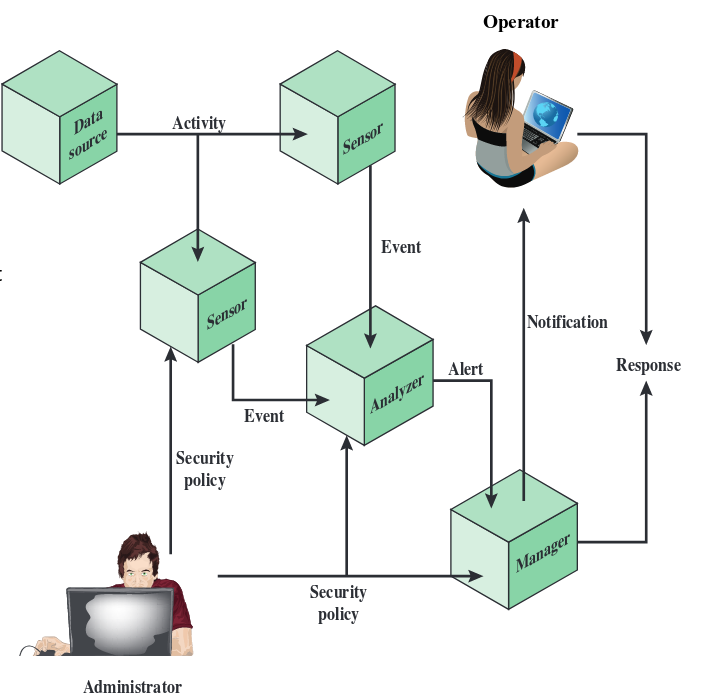
\includegraphics[width=\textwidth, height=0.85\textheight,keepaspectratio]{img/IDS.png}
		\end{figure}
	\end{frame}
	
	\begin{frame}
		Intrusion Detection System can be characterized on the basis of 2 aspects: the \emph{basing} of the system:
		\begin{itemize}
			\item Host-Based IDS
			\item Network-Based IDS
			\item Hybrid (Distributed) IDS
		\end{itemize}
		and on the techniques used for \emph{detection}:
		\begin{itemize}
			\item Signature-Based IDS
			\begin{itemize}
				\item[$\rightarrow$] We define a set of \emph{rules} that captures malicious behaviours
			\end{itemize}
			\item Anomaly-Based IDS
			\begin{itemize}
				\item[$\rightarrow$] We define the \emph{normal behaviours} and measure how close are the observed activities with respect to the model produced
			\end{itemize}
		\end{itemize}
		Can you see where Statistical Learning comes in? :)
	\end{frame}
	
	\begin{frame}
		Anomaly-Based IDS can use techniques based on Multivariate Analysis or Statistical Learning to develop the model of users' \emph{normal behaviour}\newline\newline
		Decision Trees are a good candidate for predictions since empirical results showed that this technique is one of the most accurate for intrusion detection\newline\newline
		Of course there are some drawbacks as:
		\begin{itemize}
			\item Data Gathering
			\begin{itemize}
				\item[$\rightarrow$] If you're not willing to use Stateful Protocol Analysis (i.e. you buy data from authorized vendors in order to build the model), you need sensors for data acquisition and you have to do some preprocessing
			\end{itemize}
			\item False-Positive/False-Negative rates
			\begin{itemize}
				\item[$\rightarrow$] Since intrusions are considered \emph{rare} (but often \emph{catastrophic}) events, we want to achieve the maximum accuracy possible
			\end{itemize}
		\end{itemize}
	\end{frame}
	
	\begin{frame}
		\begin{center}
			\begin{Huge}
				ANALYZER IMPLEMENTATION
			\end{Huge}
		\end{center}
	\end{frame}
	
	\begin{frame}
		\begin{itemize}
			\item An \emph{analyzer} for IDSs is a (typically) software module that collects data and raises an alarm if an intrusion is detected
			\item In this work, an hybrid Python/R software was developed:
			\begin{itemize}
				\item[1)] All the Preprocessing was done in Python for comodity (I'm quite familiar with it) and for the numbers of libraries available for Machine Learning
				\item[2)] The Decision Tree was built with R, using the rpart package
				\item[3)] Since R can work as a server to communicate with other process, there's no drawback on splitting modules using different languages (actually, this is often a requirement in software engineering!)
			\end{itemize}
			\item Data Analysis is a critical factor for achieving an high level of accuracy, thus multiple techniques were used for the process
		\end{itemize}
	\end{frame}
	
	\begin{frame}
	\vspace{0.5cm}
		Features' values in the dataset consist of heterogeneous types: we have integers, floats, strings\dots\newline\newline
		The first step is to convert all the values to a numeric type in order to proceed with the analysis! This is a very simple procedure an can be implemented straightforward by checking all the strings in the dataset
			\begin{figure}
				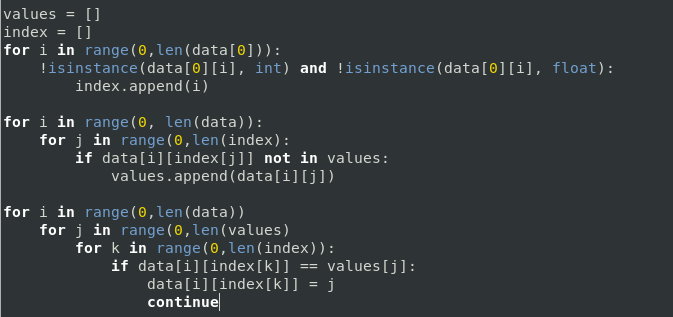
\includegraphics[width=\textwidth,height=0.85\textheight,keepaspectratio]{img/PreprocessCode.png}
			\end{figure}
	\end{frame}
	
	\begin{frame}
		The next step is features' standardization.\newline\newline This step is mandatory since Principal Component Analysis was used as a method for features' selection:
		\begin{center} If data are not standardized (i.e. scaled in order to associate to each feature a distribution with mean = 0 and variance = 1), there will be some features that appears to be the most relevant only because their values are of different scales\end{center}
		 (e.g. error rates, or rates in general usually shrink [0,1], while durations, number of requests etc are positive natural numbers)\newline\newline
		 \begin{itemize}
		 	\item[$\times$] The very important thing in this step is that we need to standardize both the test and the train set, which consists of different features' values, using the same criteria
		 	\item[$\bigstar$] Luckily for us, there is a Python library that implements all these operations for us: the Pandas library
		 \end{itemize}
	\end{frame}
	
	\begin{frame}
		\begin{figure}
			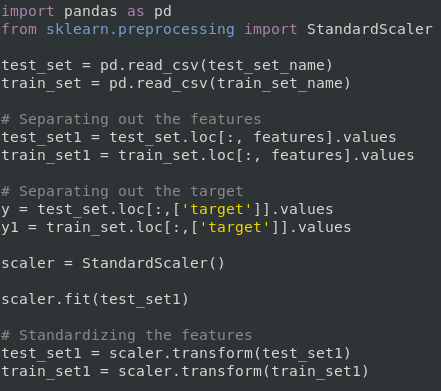
\includegraphics[width=\textwidth,height=0.8\textheight,keepaspectratio]{img/Normalization.png}
		\end{figure}
	\end{frame}
	
	\begin{frame}
		After data have been standardized, we need to select only the relevant features in the dataset (since it consists of 40 variables!)\newline\newline
		To do so, a Principal Component Analysis was conducted on the dataset.
		\begin{block}{PCA}
			\begin{itemize}
			
				\item It is a technique that uses algebra calculations to reduce the number of variables in a dataset
				\item First of all, the variance-covariance matrix $V$ must be computed
				\item Then, we need to calculate its eigenvectors and eigenvalues, that translates into solving the equation: $det( V - \lambda I) = 0$
				\item These vectors represent "new" features that explain the variance of the variables in the dataset
				\item You then choose the number of components (the vectors) you need to preserve the accuracy of the representation of the original dataset
			\end{itemize}
		\end{block}
	\end{frame}
	
	\begin{frame}
		Here we have the same problem we had with standardization: if we perform some transformation on the train-set, the \emph{same} transformation must be done on the test-set and on the real data you will gather from sensors.\newline\newline
		Luckily, again, the Pandas library comes in help:
		\begin{figure}
			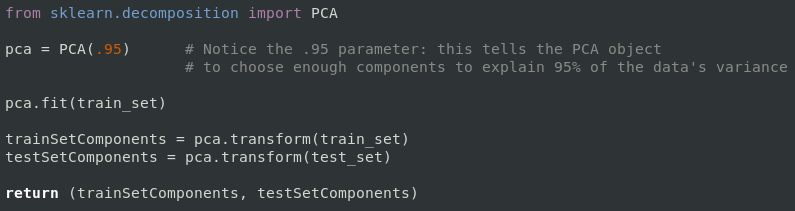
\includegraphics[width=\textwidth,height=\textheight,keepaspectratio]{img/PCA.png}
		\end{figure}
	\end{frame}
	
	\begin{frame}
		Now that data are cleaned, standardized and the principal components were calculated, we can start building the Decision Tree!\newline\newline
		Decision Trees are statistical models that can be used for classification and the analysis of variance.\newline\newline
		In this research we are most interested in classification since we want to classify \emph{bad} and \emph{good} users. In the next block is briefly described the algorithm to build a DT
		\begin{block}{Decision Tree Construction}
			\begin{itemize}
				\item For each variable we split the dataset in 2 groups (e.g. using the Gini Index metric)
				\begin{itemize}
					\item[$\rightarrow$] Since our variables are continuous, splits will be done on boolean conditions, that is: given a threshold \emph{t}, we will check the features whose value is greater than \emph{t} and the ones lower than \emph{t}
				\end{itemize}
				\item The variable (feature) that produced the "best" score will be the very first split (i.e. the root of the tree)
				\item The algorithm now proceeds recursively on each node, until a certain alt condition is met (e.g. all the variables have been chosen for splitting the dataset)
			\end{itemize}
		\end{block}
	\end{frame}
	
	\begin{frame}
		The DT was built using R, since it is faster than Python and, if our train-set is about 200 MB, our test-set is 2 GB, so considerations on performances led me thowards R\newline\newline
		Decision Trees can be built using the package \emph{rpart}. It offers many parameters to tell the algoirthm how to build it such as the variables that need to be considered and the complexity parameter (i.e. the tree \emph{depth})\newline\newline
		It also provides a function for predictions over a dataset. The output of this predictions are used to compute the \emph{Confusion Matrix}
		
\begin{center}
	{\setlength{\extrarowheight}{20pt}
	\begin{tabular}{| c | c  c |}
	\hline
		 & Actual values & \\ \hline
		Predictions & True & False  \\ \hline
		True & True Positive & False Positive \\ \hline
		False & False Negative & True Negative \\ 
		\hline
	\end{tabular}}\par
	\bigskip
	
	\begin{tiny}
		Simple $2x2$ confusion matrix example
	\end{tiny}
	\end{center}
	\end{frame}
	
	\begin{frame}
		The confusion matrix can be used to calculate the accuracy of predictions over a dataset. The formula is quite straightforward and is shown, together with the tree construction, in the figure below:
		
		\begin{figure}
			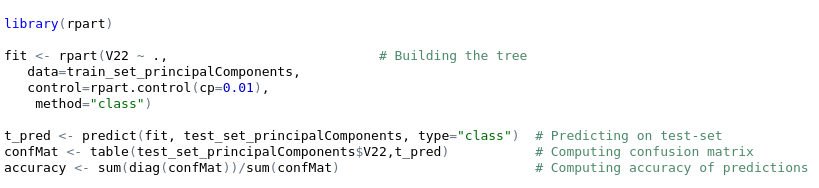
\includegraphics[width=\textwidth,height=\textheight,keepaspectratio]{img/Rpart.png}
		\end{figure}
	\end{frame}
	
	\begin{frame}
		\begin{center}
			\begin{Huge}
				RESULTS \& CONCLUSIONS
			\end{Huge}
		\end{center}
	\end{frame}
	
	\begin{frame}
		The Decision Tree was built using different three different representation of the same train-set.\newline\newline
		The Kddcup99 dataset provides a file which consists of a 10\% of the original dataset (the rows in this smaller dataset are not contiguous in the original dataset)\newline\newline
		For technical reasons, this small file was used as a train-set (usually train-sets are about the 70/80\% of the original file)\newline\newline
		For complexity parameters equal to 0.01, 0.0025 and 0.001, the algorithm was given as input:\newline
		\begin{itemize}
			\item[1)] The preprocessed dataset (i.e. strings are replaced and values are standardized, all the features in input)
			\item[2)] The features \emph{selected} by PCA (this is, indeed, a non-standard use of PCA)
			\item[3)] The new features \emph{produced} by PCA
		\end{itemize}
	\end{frame}
	
	\begin{frame}
		\begin{center}
	{\setlength{\extrarowheight}{20pt}
	\begin{tabular}{| c | c | c | c |}
	\hline
		Complexity parameter & 0.01 & 0.0025 & 0.001 \\ \hline
		StandardizedKddcup & 0.9870385 & 0.9832191 & 0.9843356 \\ \hline
		KddcupPrincipalFeatures & 0.9849946 & 0.9948412 & 0.9963878 \\ \hline
		PCA eigenvectors & 0.9901552 & 0.9951242 & 0.9956888 \\ 
		\hline
	\end{tabular}}
\end{center}
	\end{frame}
	
	\begin{frame}
		\begin{block}{Standardized Kddcup}
			\begin{itemize}
				\vspace{0.3cm}
				\item The Decision Tree ran over the whole set of features, is the one with the lowest accuracy
				\vspace{0.3cm}
				\item This Tree is also very susceptible to the complexity parameter: bigger trees mean lower accuracy (as you could see from the previous table)
				\vspace{0.3cm}
				\item Trees built with this dataset are also very much unbalanced with respect to the others
				\vspace{0.3cm}
			\end{itemize}
		\end{block}
	\end{frame}
	
		\begin{frame}
		\begin{block}{Restricted Feature Set Standardized Kddcup}
			\begin{itemize}
				\vspace{0.3cm}
				\item This train-set consist of the features chosen by the PCA, but the values used are the ones of the \emph{original} dataset
				\vspace{0.3cm}
				\item Despite the fact that this is not the standard usage of PCA, these trees show pretty good accuracy (actually, greater complexity lead to higher accuracy with respect to PCA trees)
				\vspace{0.3cm}
				\item However, this could be a consequence of using only the 10\% of the original dataset as a train-set
				\vspace{0.3cm}
				\item Regarding the Tree Structure, these ones are very similar to the PCA trees
				\vspace{0.3cm}
			\end{itemize}
		\end{block}
	\end{frame}
	
	\begin{frame}
		\begin{block}{PCA features}
			\begin{itemize}
				\vspace{0.3cm}
				\item The last train-set is the output of the PCA algorithm
				\vspace{0.3cm}
				\item The drawback of this approach is that, since we changed the original features' set, we have to transform the test-set, as well as any other value that will be used for future predictions (remember we had to \emph{fit} the PCA object in Pandas?)
				\vspace{0.3cm}
				\item The accuracy of these trees is similar to the previous one, but the gain in accuracy is lower when we increase the complexity (i.e. decrease the complexity parameter)
				\vspace{0.3cm}
				\item Just like the previous trees, these ones are very well balanced and do not suffer bigger structures
				\vspace{0.3cm}
			\end{itemize}
		\end{block}
	\end{frame}
	
	\begin{frame}
		***TREE PLOTS***
	\end{frame}
	
	\begin{frame}
		\begin{center}
			\begin{Huge}
				THANKS FOR YOUR ATTENTION
			\end{Huge}
		\end{center}
	\end{frame}
	
	
\end{document}